\documentclass[a4paper, 10pt]{article} 

\usepackage{graphicx}
\graphicspath{ {./images/} }
\usepackage{wrapfig}

\addtolength{\hoffset}{-2.25cm}
\addtolength{\textwidth}{4.5cm}
\addtolength{\voffset}{-3.25cm}
\addtolength{\textheight}{5cm}
\setlength{\parskip}{0pt}
\setlength{\parindent}{0in}

%----------------------------------------------------------------------------------------
%	PACKAGES AND OTHER DOCUMENT CONFIGURATIONS
%----------------------------------------------------------------------------------------

\usepackage{blindtext} % Package to generate dummy text
\usepackage{charter} % Use the Charter font
\usepackage[utf8]{inputenc} % Use UTF-8 encoding
\usepackage{microtype} % Slightly tweak font spacing for aesthetics
\usepackage[english, ngerman]{babel} % Language hyphenation and typographical rules
\usepackage{amsthm, amsmath, amssymb} % Mathematical typesetting
\usepackage{float} % Improved interface for floating objects
\usepackage[final, colorlinks = true, 
            linkcolor = black, 
            citecolor = black]{hyperref} % For hyperlinks in the PDF
\usepackage{graphicx, multicol} % Enhanced support for graphics
\usepackage{xcolor} % Driver-independent color extensions
\usepackage{marvosym, wasysym} % More symbols
\usepackage{rotating} % Rotation tools
\usepackage{censor} % Facilities for controlling restricted text
\usepackage{listings, style/lstlisting} % Environment for non-formatted code, !uses style file!
\usepackage{pseudocode} % Environment for specifying algorithms in a natural way
\usepackage{style/avm} % Environment for f-structures, !uses style file!
\usepackage{booktabs} % Enhances quality of tables
\usepackage{tikz-qtree} % Easy tree drawing tool
\tikzset{every tree node/.style={align=center,anchor=north},
         level distance=2cm} % Configuration for q-trees
\usepackage{style/btree} % Configuration for b-trees and b+-trees, !uses style file!
\usepackage[backend=biber,style=numeric,
            sorting=nyt]{biblatex} % Complete reimplementation of bibliographic facilities
\addbibresource{ecl.bib}
\usepackage{csquotes} % Context sensitive quotation facilities
\usepackage[yyyymmdd]{datetime} % Uses YEAR-MONTH-DAY format for dates
\renewcommand{\dateseparator}{-} % Sets dateseparator to '-'
\usepackage{fancyhdr} % Headers and footers
\pagestyle{fancy} % All pages have headers and footers
\fancyhead{}\renewcommand{\headrulewidth}{0pt} % Blank out the default header
\fancyfoot[L]{} % Custom footer text
\fancyfoot[C]{} % Custom footer text
\fancyfoot[R]{\thepage} % Custom footer text
\newcommand{\note}[1]{\marginpar{\scriptsize \textcolor{red}{#1}}} % Enables comments in red on margin

%----------------------------------------------------------------------------------------

\rfoot{MSc DS-AI Université Côte d'Azur, \LaTeX\, Report - Page \thepage}
\begin{document}

%-------------------------------
%	TITLE SECTION
%-------------------------------

\fancyhead[C]{}
%\hrule \medskip % Upper rule
\begin{minipage}{0.24\textwidth} 
\raggedright
\footnotesize
Quentin Le Roux \hfill
\end{minipage}
\begin{minipage}{0.5\textwidth} 
\centering 
\begin{center}
    Summary seminar 1 -- Histopathology
\end{center}
\end{minipage}
\begin{minipage}{0.245\textwidth} 
\raggedleft
\today
\end{minipage}
\hrule 
\bigskip

%-------------------------------
%	CONTENTS
%-------------------------------

This seminar covered an \textbf{introduction to machine learning for histopathology}, presented by \textit{Paul Tourniaire} from the 3iA Côte d'Azur Institute. 
\newline\newline
Histopathology is a gold standard of cancer treatment diagnosis procedures. As part of the French multidisciplinary diagnosis framework "RCP", pathologists play a key role in charting treatment protocols for patients, using key data and information such as tumor sizes, metastases, nodes, etc. With the rapid growth of AI in fields such as healthcare, a question arose in histopathology:

\begin{center}
\textit{Can AI help pathologists diagnose cancer and assign the best treatments}?
\end{center}

\section{The Research's Goal}
The research is undergone by P. Tourniaire, H. Delingette, M. Ilié, P. Hofman, and N. Ayache. It aims at developing an \textbf{AI-based imaging and biological data analyzer}. I.e. A neural network that can process and infer from biomarkers so as to better select therapy avenues for Non Small Cell Lung Cancers (abbr. NSCLC). 

The current state of research has already resulted in a multi-modal model that is successful in predicting immunotherapy responses. The next step is to expand the model to predict a treatment's chance of success based on a defined set of biomarkers.

\section{Data Availability and Use}

\begin{wrapfigure}{r}{0.25\textwidth} %this figure will be at the right
    \centering
    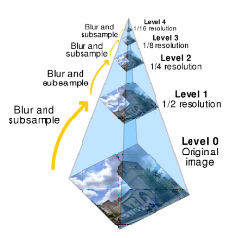
\includegraphics[width=0.2\textwidth]{pyramid}\\
    {\scriptsize Figure 1: Pyramidal Image Structure}
\end{wrapfigure}

Biopsy and resections are the main ways to produce histopathological data. Tissues are sliced and stained using color agents (e.g. hematoxylin) that helps researchers create digitized slides: \textbf{high resolution multi-level pictures in a single digitized file format called a HES Whole Slice Image (WSI), or \texit{pyramidal file}} (see Fig. 1).

This format holds multiple magnifications for varying levels of analysis. To process the data, researchers have access to both generic (e.g. scikit-learn, PIL) and dedicated (e.g. openslide, pyvips) Python libraries for computer vision.

As part of the project, two other types of data are used: IHC slides, and bionomics.

\section{Issues and Challenges of Using WSI}

WSI are large files that cannot be processed at once. A \textbf{tiling approach is almost always necessary}. Thanks to the different magnifications and the tiling, a so-called multiple-instance learning (MIL) is possible. WSI are not normalized, and show multiple colour discrepancies and many types of artefacts (e.g. folds, tears). A strong pre-processing phase is thus necessary.

\section{Data Pipeline and Models}

Slides are pre-processed using multiple, successive methods (see Fig. 2). More complex combinations of image filters and classifiers can be applied (e.g. HistoQC). Once pre-processed, images are fed into a model.
\\
\begin{wrapfigure}{r}{0.7\linewidth}
\centering
\fbox{\parbox[t]{5em}{{\scriptsize First task\\\\Grayscaling\\Thresholding}}}%
\raisebox{-4ex}{$\to$}%
\fbox{\parbox[t]{8.5em}{{\scriptsize Second Task\\\\filter out noisy elements}}}%
\raisebox{-4ex}{$\to$}%
\fbox{\parbox[t]{4.5em}{{\scriptsize Third Task\\\\Tiling}}}
\raisebox{-4ex}{$\to$}%
\fbox{\parbox[t]{8em}{{\scriptsize Fourth Task\\\\Staining Normalization (macenko method)}}}
\\{\scriptsize Figure 2: Pre-processing Pipeline}
\end{wrapfigure}

Three models were covered: \textbf{CLAM} (ResNet50 performing feature extraction followed by Multi-Class Attention Branches that yields an attention score), \textbf{MIL+RNN} (classifier RNN outputting slide targets), \textbf{CHOWDER} (uses local descriptors and a CNN to output classifier predictions). Performance is checked via an Area-under-the-Curve (AUC) metric using mean-pooling as a baseline.

\section{Conclusion}

Computational histopathology has now reached human-comparable results on cancer related tissues in many different tasks (e.g. tumour classification, survival prediction). The future is bright for RCPs.
\end{document}

%doc by Quentin Le Roux